\documentclass{acm_proc_article-sp}

\usepackage{listings}
\usepackage{color}
\usepackage{subfigure}

\definecolor{lightgray}{rgb}{.9,.9,.9}
\definecolor{darkgray}{rgb}{.4,.4,.4}
\definecolor{purple}{rgb}{0.65, 0.12, 0.82}

\lstdefinelanguage{JavaScript}{
  keywords=[1]{typeof, new, catch, function, return, for, switch, var, if, in, while, do, else, case, break},
  keywordstyle=[1]\color{blue}\bfseries,
  keywords=[2]{this, document, window, null, true, false},
  keywordstyle=[2]\color{green}\bfseries,
  identifierstyle=\color{black},
  sensitive=false,
  comment=[l]{//},
  morecomment=[s]{/*}{*/},
  commentstyle=\color{purple}\ttfamily,
  stringstyle=\color{red}\ttfamily,
  morestring=[b]',
  morestring=[b]"
}

\lstset{
   language=JavaScript,
   backgroundcolor=\color{lightgray},
   extendedchars=true,
   basicstyle=\footnotesize\ttfamily,
   showstringspaces=false,
   showspaces=false,
   tabsize=2,
   breaklines=true,
   showtabs=false,
   captionpos=b,
   columns=fullflexible
}

\begin{document}
\title{Developing a Random Terrain Generator}
\numberofauthors{2}
\author{
  \alignauthor Zhongpeng Lin \\
  \affaddr{UC Santa Cruz} \\
  \email{linzhp@soe.ucsc.edu}
  \alignauthor Huascar A. Sanchez \\
  \affaddr{UC Santa Cruz} \\
  \email{hsanchez@cs.ucsc.edu}
}

\maketitle
\begin{abstract}
The aim of this paper is to describe a system that combines three well-known terrain generation algorithms (i.e., Perlin Noise, Simplex Noise, and the Diamond Square algorithms), and a JavaScript 3D engine, called Three.js. Our Web-based terrain generator performs terrain generation in two steps. First, it randomly pick the algorithm that will set the world. Second, our terrain generator tool applies a few visual effects (e.g., fog) and animations on objects part of the generated world to create a sense of immersion for users interacting with our tool. Our tool allows a full first-experience of a realistic, interactive virtual environment by means of some basic navigation operations, such as world rotation, and world navigation (e.g., moving forward, moving backwards, moving to the left, and moving to the right). 
\end{abstract}

\category{H.4}{Information Systems Applications}{Miscellaneous}
\category{D.2.8}{Software Engineering}{Metrics}[complexity measures, performance measures]

% TODO (whoever) change to the apropropriate terms..
\terms{Algorithms, Terrain, Procedural-Content-Generation} 

\keywords{Terrain Generator, Three.js, WebGL} 

\section{Introduction} % (fold)
\label{sec:introduction}

In recent years, the advances in processing power of average home computers have made it possible to simulate realistic terrains near-realtime. This paper presents a method that combines three well-known terrain generation algorithms (i.e., Perlin Noise  \cite{perlin:2002}, Simplex Noise \cite{perlin:2001}, and Diamond Square \cite{fournier:1982}) and a Javascript 3D engine, called Three.js \cite{threeJS}, for generating natural looking terrains on the Web. With some criteria for applicability in robot designs generation, a Web-based tool for randomly generating terrains is then presented. Finally, to create more interesting and complicated terrains, We mixed the noise and fractal functions of these well-known algorithms.     

We care about procedural terrain generation for different reasons. To name a few, one aspect of our robot design generator project at the Augmented Design Lab is the testing of whether the produced designs are valid. Consequently, performing a drive-test of those design on numerous simulated (procedurally generated) terrains will be a great validity test for our designs. Additionally, art assets such as terrain's textures and geometry are difficult and time consuming to generate. Consequently, by using procedural terrain generation techniques, We will be able to create many such assets with subtle modifications of parameters. Lastly, since this is a Web-based tool, We need to deal with lots of terrain variations and memory/bandwidth requirements. Therefore, We believe the use of procedural terrain generation techniques to satisfy those requirements is the logical choice.    

In the algorithms described in this paper, terrain will be represented by three-dimensional height maps using floating point values between 0 and 1. Unless otherwise stated, all examples explained in this paper use the respective default noise or fractal functions of the used terrain generation algorithms. All implementations of these algorithms, as well as the overall tool, were done in Javascript.  

This paper is structured as follows: First, We briefly review the related work. Then, We describe the overall terrain generation system and write about the tool's architecture, the specific choices we made in implementing not only the Perlin Noise, Simplex Noise, and Diamond algorithms, but also the overall tool. Finally, We conclude and then talk about the future work.  

% section introduction (end)

\section{Related Work} 
\label{sec:related_work}

There has been a large amount of research in the area of terrain generation. Traditionally most of it has focused on generating terrain by using fractal techniques, like Olsen's \cite{lechner:2006}, Szeliski and Terzopoulos's \cite{szeliski:1989}, and Pi's \cite{pi:2006}.

Olsen \cite{lechner:2006} discussed the use fractal Brownian motion and perturbed Voronoi diagrams in erosion algorithms. Szeliski and Terzopoulos's \cite{szeliski:1989} used real digital elevation data which they perturb using splines to address fractal terrain generation. Pi \cite{pi:2006} created fractal landscapes using Perlin noise. As with most fractal-based approaches, their algorithms do not appear to be controllable.

Li, Wang, Zhou, Tang, Yang \cite{li:2006} used machine learning to model example height maps. These models were then used by the authors to come up with new interesting terrains. Unfortunately, no good deed goes unpunished. A major issue with this approach was a frequent unclearness of what needed to be learned or what features were important to be part of the training data.

Ong \cite{ong:2005} used genetic algorithms to generate terrains. Besides focusing on controllability, their approach sketched the boundary of the terrain to be generated. The main form of controllability of this approach was a database containing a set of representative height map samples, which could be controlled by the designer.
  
Lastly, Doran and Parberry \cite{doran:2010} focused on allowing the designer more natural control over the generated terrains without sacrificing too much desirable Procedural Content Generation attributes, such as novelty, structure, interest, and speed.

The aim of this paper is to provide a method that combines three well-known terrain generation algorithms (i.e., Perlin Noise  \cite{perlin:2002}, Simplex Noise \cite{perlin:2001}, and Diamond Square \cite{fournier:1982}) and a Javascript 3D engine, called Three.js \cite{threeJS}, for generating natural looking terrains on the Web.

% section related_work (end)

\section{System Overview} 
\label{sec:system}

\subsection{Problem Description}

% subsection problem description (end)

\subsection{Terrain Generator Architecture}
The architecture of our terrain generator is shown in Figure~\ref{fig:arch}. At the bottom sits the WebGL API, which is used to send shader programs to GPU. Three.js is built on WebGL API to hide details of shaders and provide a convenient way to manipulate the 3D scene. Then we developed several utility functions setup the scene and camera, as well as using the height map generated by above-mentioned algorithms to render terrains. We also develop extensions to three.js to produce richer effects. On top of them, we developed a simple API to be called from HTML page.
\begin{figure}
	\center
	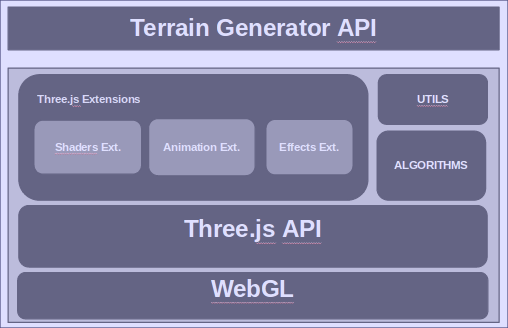
\includegraphics[scale=0.45]{arch.png}
	\caption{Architecture}
	\label{fig:arch}
\end{figure}
% subsection terrain generator architecture (end)

\subsection{Terrain Generation Algorithms}

The main goal of this section is to provide an overview of the three algorithms that were implemented in our Web-based terrain generator for synthesis of realistic-looking terrains. Traditionally, procedural terrain generation focuses on the generation of a height for each point in a 2D space. In other words, it can be seen as function that maps \textit{x} and \textit{y} coordinates into \textit{z} coordinates: \[z=terrainGen(x, y)\]

Several techniques have built upon this height generation idea to create realistic-looking landscapes.

Two types of noise-based algorithms and one type of fractal-based algorithms are examined in this section, namely Perlin Noise (sometimes referred to as Perlin ``Classic'' Noise), Simplex Noise, and the Diamond Square algorithms. The first two were first described by Ken Perlin \cite{perlin:2002}, \cite{perlin:2001}, and the last one by Fournier, Fussell, and Carpenter \cite{fournier:1982}. These algorithms have since established themselves as a base from which various improvements have
been suggested \cite{ong:2005, lechner:2006, pi:2006, li:2006, doran:2010} in the  procedural terrain generation field. An overview of each type is provided in the following subsections. 

\subsubsection{Perlin Noise}
The Perlin Noise is a procedurally generated visual effect developed by Ken Perlin \cite{perlin:2002}. It is a technique very useful in circumstances where computer memory is limited and users want to simulate elements from nature. The Perlin Noise works as follows:

\begin{enumerate}
\item It begins by creating a grid of vectors (gradients).
\item Each grid point has a gradient pointing away from it in a random direction (Figure~\ref{fig:randomGradients}).
\item For any given point (or pixel), interpolate the value from the surrounding N gradients. For a 2D space, the $N \eq 4$.
\item Finally, sum all values of the interpolations. Some example graphs generated by Perlin noise are show in Figure~\ref{fig:perlinEg}.
\end{enumerate}

Perlin noise can be created in 3D and higher dimensions. How do you do that? Well, you actually take slices along the z axis. Almost like a brain scan. You have a big 3D blob of noise and you just take thin slices and look at each one. Since each slice only changes a little, then it it looks like each slice animates all nicely.

\begin{figure}
	\center
	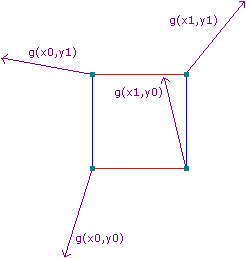
\includegraphics[scale=0.5]{images/gradients.png}
	\caption{Random Gradients}
	\label{fig:randomGradients}
\end{figure}
\begin{figure}
	\center
	\subfigure{
		
\includegraphics[scale=0.5]{images/woodgrain.png}
	}
	\subfigure{
		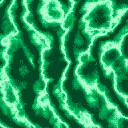
\includegraphics[scale=0.5]{images/marble.png}
	}
	\subfigure{
		
\includegraphics[scale=0.5]{images/clouds.png}
	}
	\caption{Perlin Noise Examples}
	\label{fig:perlinEg}
\end{figure}

The next algorithms to be described is the Simplex noise algorithm, which was developed by Ken Perlin \cite{perlin:2001} to overcome of the problems of the classic Perlin Noise.

\subsubsection{Simplex Noise}
Simplex noise is another noise generation algorithm developed by Perlin \cite{perlin:2001}. The goal of this algorithm is to make the noise generation simpler and faster, so that it could be implemented on hardware. In contrast to the Perlin's classic noise algorithm, the Simplex noise can scale to higher dimensions (4D, 5D and up) with much less computational cost. 

In 2D space, simplex noise differs from Perlin noise in the following ways:
\begin{enumerate}
	\item It uses a grid consisting of equilateral triangles instead of squares. As a result, there are only three adjacent grid points for each point in the space.
	\item Summation is used instead of interpolation. Simplex noise sums up the contributions from each corner (grid point) of the triangle, where ``the contribution is a multiplication of the extrapolation of the gradient ramp and a radially symmetric attenuation function'' \cite{Gustavson2005}. The calculation of summation is much less than interpolation, making simplex noise faster.
\end{enumerate}

Another approach for simulating realistic-looking landscapes is the diamond-square algorithm. Briefly, this algorithm is a midpoint displacement method that works by recursively calculating the missing values halfway among already known values and then randomly offsetting the new values inside a range, which has been determined by the current recursion depth. More details of this algorithm are described in the following subsection.

\subsubsection{Diamond-Square}
The Diamond-square algorithm is another method for generating height maps of artificial terrains. The difference between this algorithm and the above mentioned ones is that this algorithm uses fractals. 

This algorithm works on a 2D array of points; the number of points in each dimension should be $2^{n} + 1$, where $n$ is an integer. For example, $17 \times 17$, $1025 \times 1025$, etc). The algorithm starts by assigning seed values as heights to the four corners of a square, then it starts its iterative subdivision routine in two steps:

\begin{itemize}
	\item \textbf{The diamond step:} Average the heights of the four corners, add it to a random value and then assign the sum as the height of the square \textit{midpoint}, where two diagonals meet. The midpoints and corners form diamond shapes in the grid.
	\item \textbf{The square step:} Take each diamond of four points, average the heights of them and then add it to a random value in the same range of previous step to get the sum. Assign the sum to the midpoint of the diamond as the height. Once this done, it gives smaller squares again.
\end{itemize}

The iteration can repeat until all points in the grid have heights (Figure~\ref{fig:dsa}).

\begin{figure}
	\center
	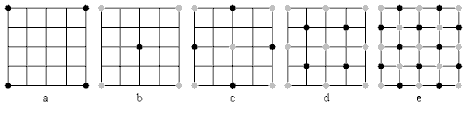
\includegraphics[scale=0.5]{images/dsa.png}
	\caption{Diamond-square Algorithm}
	\label{fig:dsa}
\end{figure}

\subsubsection{Combination of Algorithms}

Since all of the three algorithms described in this section accept \textit{x} and \textit{y} coordinates, and produce a height, we can combine these algorithms in different ways:

\begin{enumerate}
	\item Add up the height maps generated by several run of the same algorithm.
	\item Add up the height maps of different algorithms.
\end{enumerate}

By combining these algorithms, we are able to produce more interesting and complex terrains that just using individual algorithms; one at a time.

% subsection algorithms (end)

\subsection{WebGL and Three.js}

With the introduction of HTML5, experimentation with the new  \texttt{canvas} began. The \texttt{canvas} tag introduces a high performance dynamic scriptable shape rendering capability, which is very useful if doing high-quality 3D graphics or performing super fast animations on the Web without the use of plug-ins \cite{wiki:webgl}. Consequently, large number of projects being built on top of this tag started appearing. One of these projects is the 3D Javascript engine, developed by Ricardo Cabello (a.k.a., MrDoob), called Three.js.  

Three.js engine's functionality provide you with an out-of-the-box WebGL renderer (\texttt{canvas}, \texttt{svg} and WebGL), and controllable camera and viewport. The physics and animation work is up to the developer to work out. Nevertheless it is not complicated to add up these functionality to Three.js as it is shown in many Three.js examples found online at \cite{threeJS}. Figure~\ref{fig:threejs} illustrates an example of a cube rendered by Three.js.

\begin{figure}
	\center
	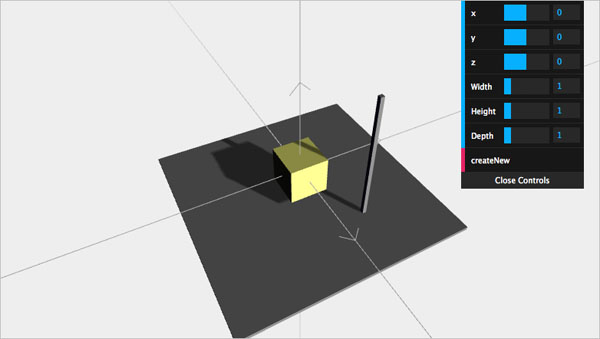
\includegraphics[scale=0.45]{images/basicsThreeJS.png}
	\caption{Three.js Example}
	\label{fig:threejs}
\end{figure}


Great examples have been created by MrDoob and by Three.js' contributors and the code is freely available. The code is relatively easy to follow and understand by even inexperienced Javascript developer. Hence, the code is released as Three.js' constantly growing documentation. 

Google Chrome is the recommended browser for doing and testing Three.js work. It is HTML5 compatible and much slightly better than FireFox, Opera, and definitely better than IE. Additionally, Chrome’s JS engine is very fast and smooth.


Three.js' basic set up is the following. First, since we are using WebGL in this project, we create an instance of \texttt{WebGL Renderer}:

\begin{lstlisting}
var renderer = new THREE.WebGLRenderer({antialias: true});
renderer.setSize(document.body.clientWidth, document.body.clientHeight);
\end{lstlisting}

Then, we plug this render in as an HTML element. We use the \texttt{body} tag as our document container:

\begin{lstlisting}
document.body.appendChild(renderer.domElement);
\end{lstlisting}

We can also include a bit of styling to make it pretty:

\begin{lstlisting}
renderer.setClearColor( scene.fog.color, 1 );
renderer.domElement.style.position = "absolute";
renderer.domElement.style.top = MARGIN + "px";
renderer.domElement.style.left = "0px";
\end{lstlisting}

To get things better, we can create an instance of a \texttt{Scene}, add some \texttt{Fog} visual effect to it, and then add a \texttt{Cube}: 

\begin{lstlisting}
var scene = new THREE.Scene();
scene.fog = new THREE.Fog(0x050505, 2000, 4000);
scene.fog.color.setHSV(0.102, 0.9, 0.825);
var cube = new THREE.Mesh(new THREE.CubeGeometry(50, 50, 50), new THREE.MeshBasicMaterial({color: 0x000000}));
cube.position.x = 30;
cube.position.y = 40;
cube.position.z = 50;
cube.rotation.x = Math.PI / 4;
scene.add(cube);
\end{lstlisting}

The above code could be then improved by adding a \texttt{Camera} object. This camera will allow us to see the cube from different angles. Technically, all we need to do is to create a \texttt{Camera} instance, set the position and orientation of such camera, and then voila! Now we have a basic interactive world consisting of a cube in the center of the \texttt{canvas}:

\begin{lstlisting}
//PerspectiveCamera(field-of-view, viewAspectRatio, nearest, farthest);
var camera = new THREE.PerspectiveCamera(45, width / height, 1, 10000);
camera.position.z = 300;
camera.lookAt(30, 40, 50);
\end{lstlisting}

Finally, the \texttt{WebGL Renderer} renders the scene from the camera. At this point, a 3D cube will appeared in the center of the screen:

\begin{lstlisting}
renderer.render(scene, camera);
\end{lstlisting} 
  
Interested readers can find more details about Three.js at \cite{threeJS}, and about WebGL at \cite{wiki:webgl}, \cite{learningWebGL}. In the next section, We will write about the algorithms we implemented in our Web-based terrain generator.

% subsection three.js (end)

\subsection{Demonstration}
In this section, we will present the interface of the terrain generator, with all the features described in previous sections. 

The system has only one web page as interface. The middle of it shows the first-person view of the terrain. Below the terrain is a simple help for users to control the view. Users could move forward/backward/right/left using the arrow keys, or press 'g' to regenerate another terrain. In addition, users could toggle day or night view by pressing 'n' key. 

Figure~\ref{fig:demo_0_1} was generated using the Perlin Noise algorithm and covered by a grass texture. We could see the surface of the terrain was very smooth, with high mountains. Figure~\ref{fig:demo_1_1}, \ref{fig:demo_1_2} and \ref{fig:demo_1_3} were generated by the Diamond-square algorithm. The difference between both generated terrains was the used texture. You could also see these terrains were not as smooth as the one generated by the Perlin Noise algorithmn. These generated terrains were mostly rolling hills. 

Figure~\ref{fig:demo_2_1} was generated by combining the Perlin Noise and Diamond-square algorithms. The generated terrain combines the terrain features of the two: high mountains with rough surface. Finally, the Simplex noise algorithm was used by our generator to generate sharp mountains as shown in Figure~\ref{fig:demo_3_0}, \ref{fig:demo_3_2} and \ref{fig:demo_3_3}.

\begin{figure*}
	\center
	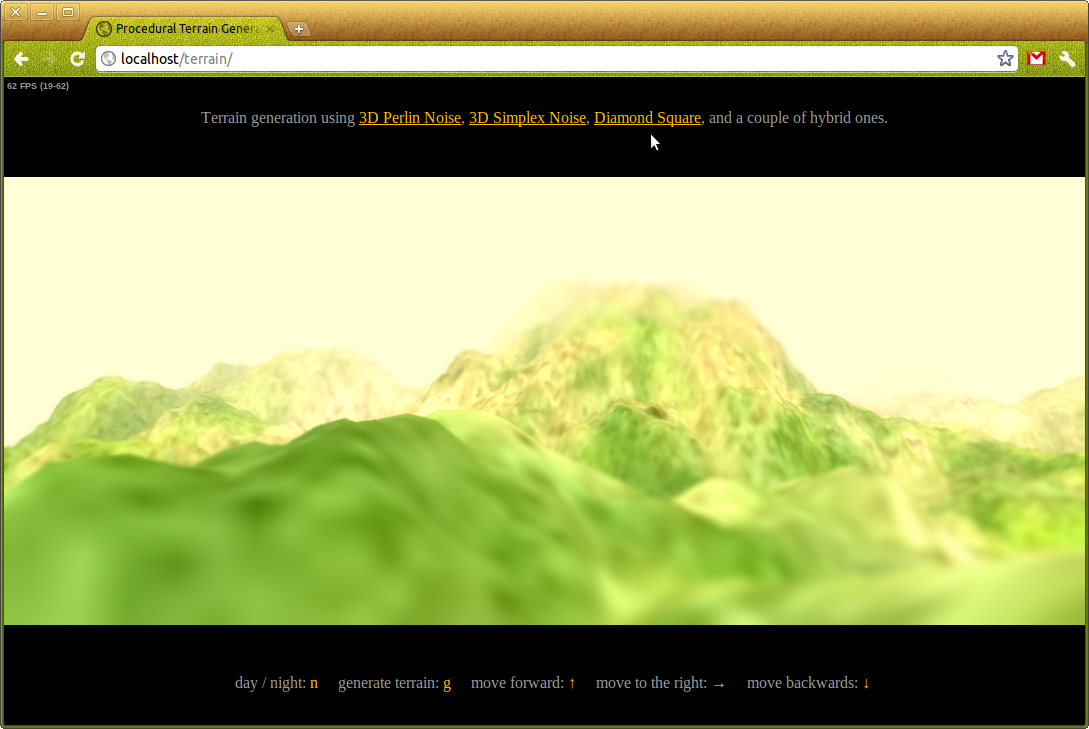
\includegraphics[scale=0.4]{images/demo_0_1.png}
	\caption{Perlin Noise with grass texture}
	\label{fig:demo_0_1}
\end{figure*}
\begin{figure*}
	\center
	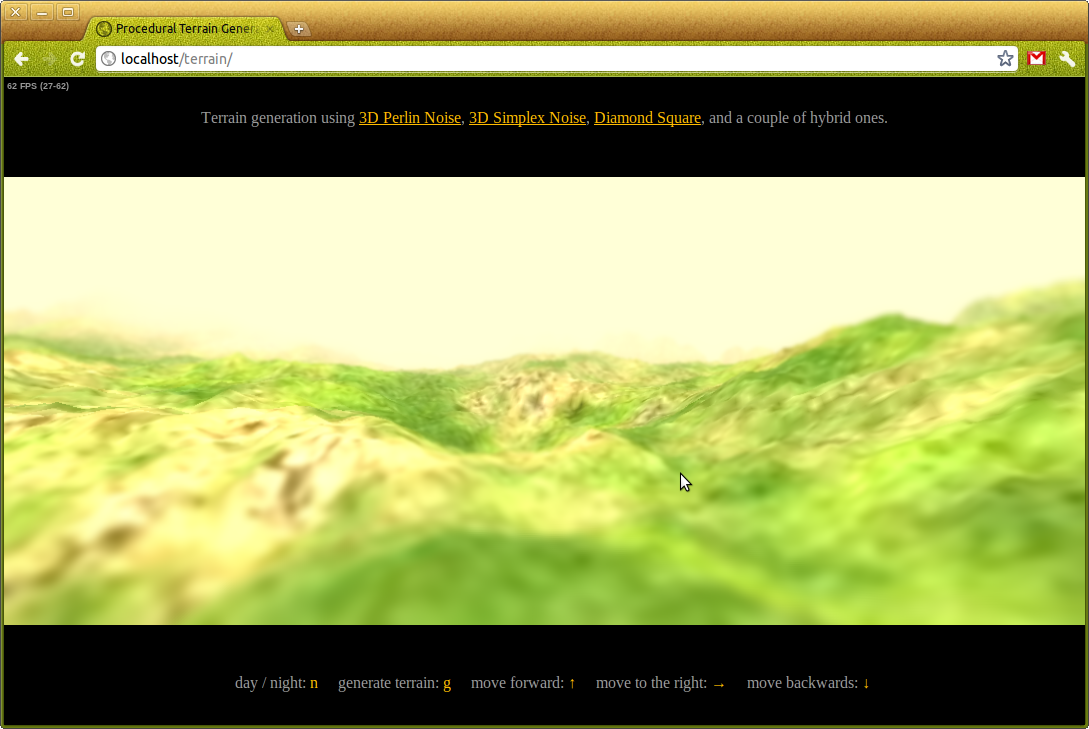
\includegraphics[scale=0.4]{images/demo_1_1.png}
	\caption{Diamond-square with grass texture}
	\label{fig:demo_1_1}
\end{figure*}
\begin{figure*}
	\center
	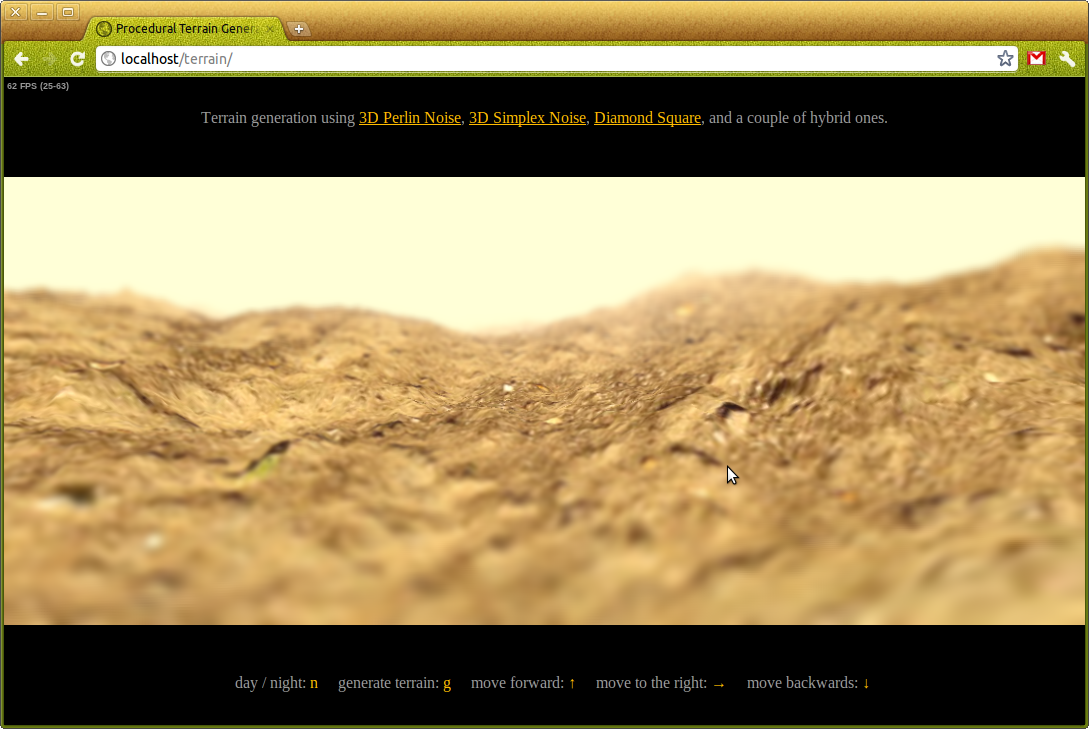
\includegraphics[scale=0.4]{images/demo_1_2.png}
	\caption{Diamond-square with sand texture}
	\label{fig:demo_1_2}
\end{figure*}
\begin{figure*}
	\center
	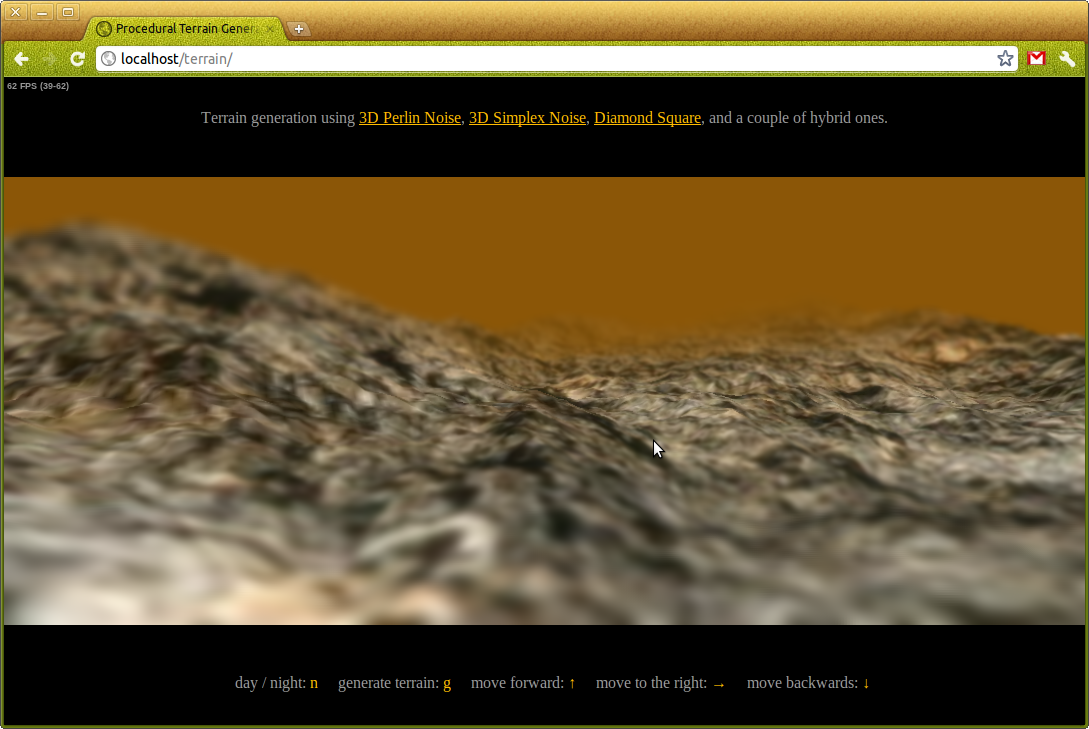
\includegraphics[scale=0.4]{images/demo_1_3.png}
	\caption{Diamond-square with rock texture}
	\label{fig:demo_1_3}
\end{figure*}
\begin{figure*}
	\center
	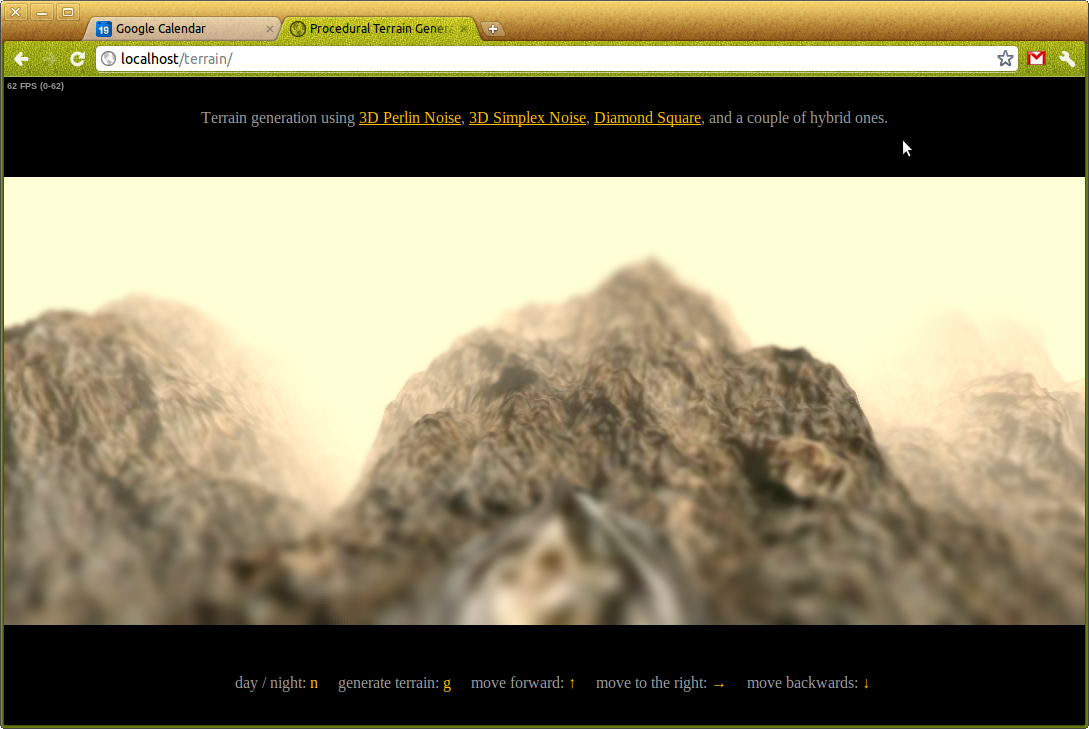
\includegraphics[scale=0.4]{images/demo_2_1.png}
	\caption{Combining Perlin noise and diamond-square with grass texture}
	\label{fig:demo_2_1}
\end{figure*}
\begin{figure*}
	\center
	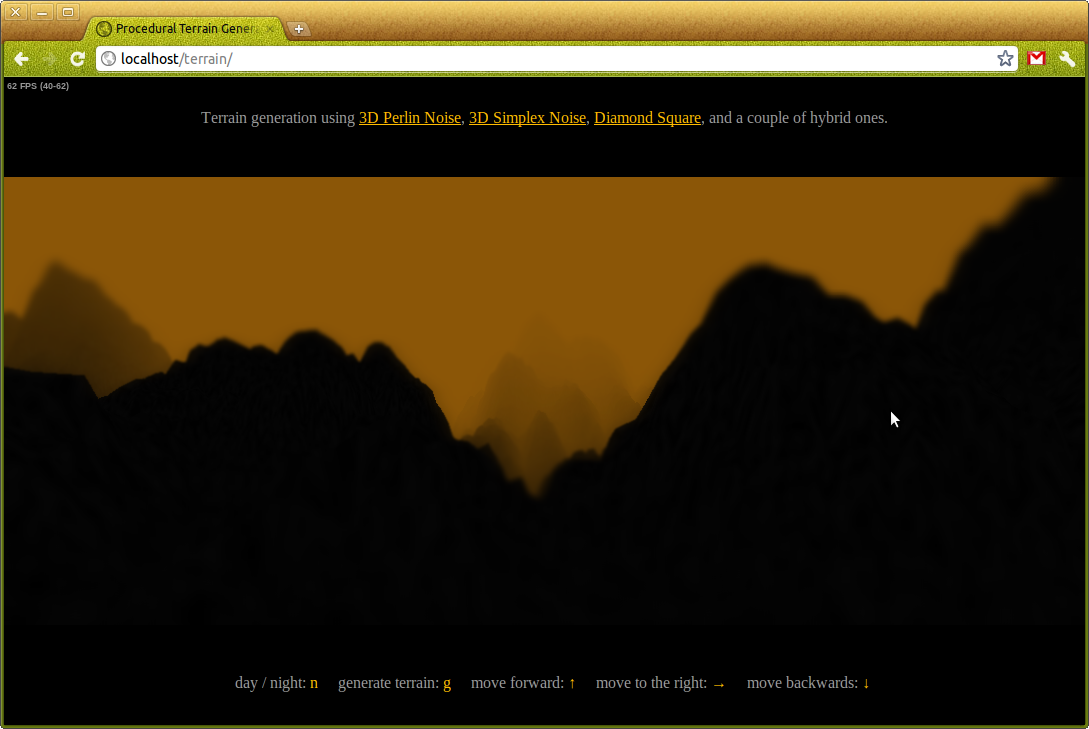
\includegraphics[scale=0.4]{images/demo_3_0.png}
	\caption{Simplex noise}
	\label{fig:demo_3_0}
\end{figure*}
\begin{figure*}
	\center
	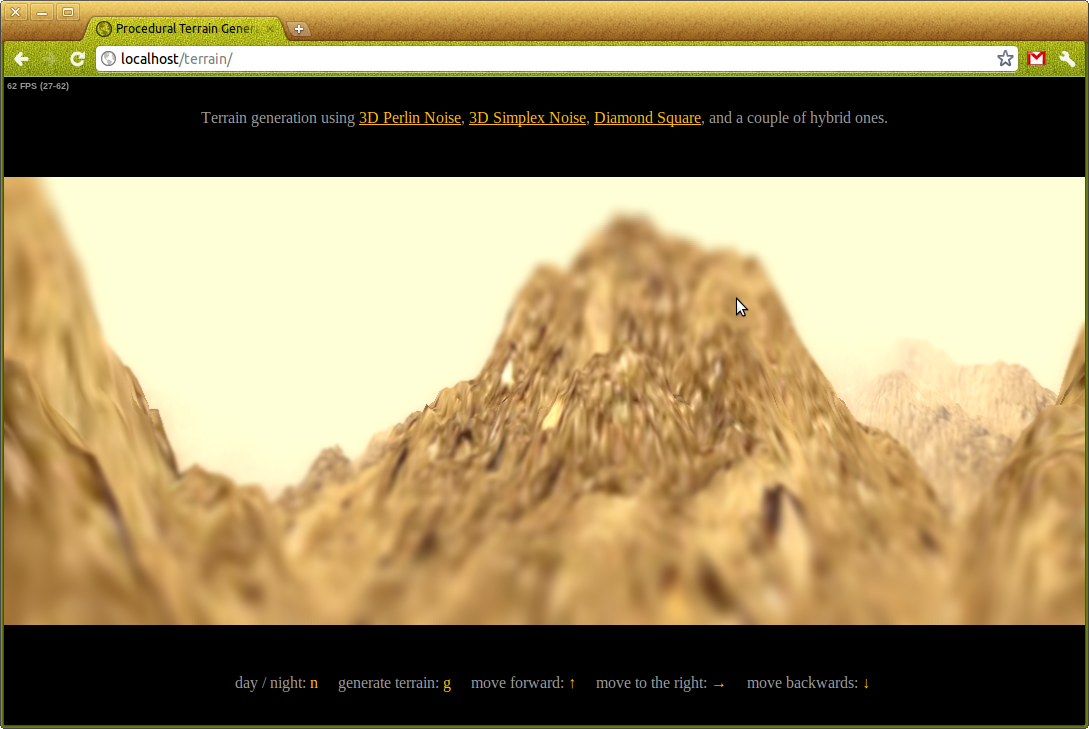
\includegraphics[scale=0.4]{images/demo_3_2.png}
	\caption{Simplex noise with sand texture}
	\label{fig:demo_3_2}
\end{figure*}
\begin{figure*}
	\center
	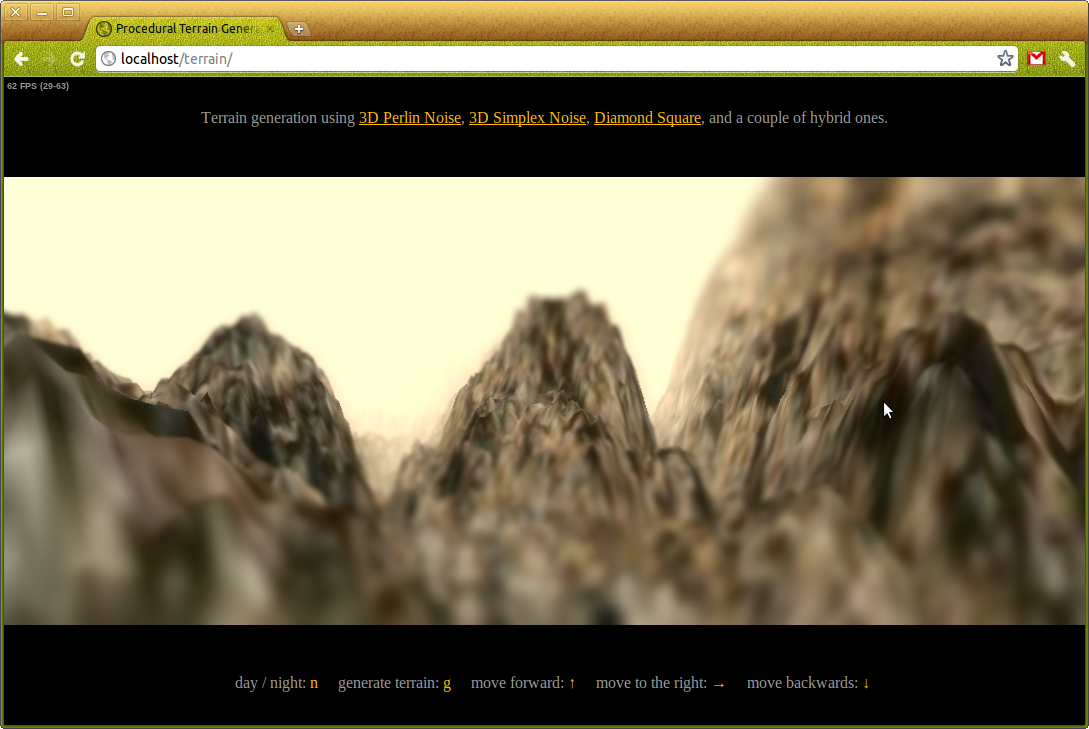
\includegraphics[scale=0.4]{images/demo_3_3.png}
	\caption{Simplex noise with rock texture}
	\label{fig:demo_3_3}
\end{figure*}
% subsection demo (end)


% section system overview (end)


\section{Conclusions} % (fold)
\label{sec:conclusions}

This paper presented a Web-based random terrain generator tool. Our demo showed all the features described in this paper and gave the audience a chance to experience the generation of different terrains based on noise functions, such as the Perlin and Simplex noise, fractal functions, such as the Diamond Square algorithm, and the combination of noise-and-fractal functions. 

Our screenshots showed that the produced terrains were indeed realistic. Without doubt the used procedural terrain generation techniques nicely scaled in our Web-based random terrain generator when generating random terrains. 

This hybrid of flexible noise and fractal functions, making use of a powerful 3D engine, may lead to more tunable terrains that could meet certain testing criteria needed to validate robot designs produced by our Robot Design Generator tool. 

Still lacking in our tool are: useful features for quickly and cogently indicating what function(s) was used to set the shape of the world, and controllable parameters that could influence the overall elevation, roughness, and local details of the generated terrains. These features would be eventually implemented and then included in the final Robot Design Generator project. 


% section conclusions (end)

\section{Future Work} 
\label{sec:future_work}
% TODO

% section future work(end)


\bibliographystyle{abbrv}
\bibliography{report}

\end{document}
